% main.tex — 济南大学硕士学位论文主文件
%
% 编译：./build.sh           （或 xelatex main.tex 跑两遍 + bibtex + 两遍）
% 产物：build/main.pdf
%
% 结构约定：
%   frontmatter/  封面、声明、中英文摘要、目录
%   chapters/     正文章节，一章一个文件
%   refs/         参考文献库
%   figures/      图
%
% 正文里每个实验数字都要能追溯到工件，来源注释写在数字旁边。
% 动笔前先读 WRITING_RULES.md。

\documentclass[UTF8, zihao=-4, openany]{ctexbook}

\usepackage{ujnthsis}
\usepackage{xeCJK}
\usepackage{hyperref}
\hypersetup{
  colorlinks = true,
  linkcolor  = black,
  citecolor  = black,
  urlcolor   = black,
  bookmarksnumbered = true,
}
\usepackage{cleveref}   % 交叉引用自动带「图/表」字样，正文写 \cref{fig:x} 即可

\thesistitle{基于 3D 高斯泼溅的动态场景 SLAM 研究}
% ↑ 题目是占位，定稿后替换（会同步到偶数页页眉）

% 参考文献走 bibtex + gbt7714（国标），不用 biblatex。
% 文献库见 refs/references.bib。

\begin{document}

% ---------------------------------------------------------------- 前置部分
\frontmatterpagenumbering
% frontmatter/cover.template.tex — 封面（占位，字段待填）
%
% 官方模板的封面字段（照抄自 02_resources/ujn_biyelunwen_muban 里的 .doc）：
%   分类号（参考《中国图书馆分类法》，查询网站 https://www.clcindex.com/）
%   学号 / 密级（公开、内部、秘密、机密、绝密）
%   「硕 士 学 位 论 文（学 术 学 位）」字样
%   中文题目（宋体小二，副标题小三，居中）、英文题目（Times 小二/小三，粗体）
%   作者姓名、导师姓名（四号 Times，粗体）
%   学科专业、研究方向、培养单位等（四号，分散对齐 / 小三楷体）
%   日期
%
% 这一页最终交付时建议在 Word 里对着官方 .doc 排版，或等我们把封面字段
%    全部核对完再数字化成 LaTeX。现在先用一个能编译的占位版。

\begin{titlepage}
\centering
\vspace*{2cm}

{\heiti\zihao{2} 硕 士 学 位 论 文}\\[0.3cm]
{\heiti\zihao{3}（学 术 学 位）}\\[2cm]

{\songti\zihao{2} 基于 3D 高斯泼溅的动态场景 SLAM 研究}\\[2cm]

\begin{spacing}{1.8}
{\songti\zihao{4}
\begin{tabular}{rl}
学\quad\quad 号 & \underline{\makebox[5cm]{}} \\
论文作者 & \underline{\makebox[5cm]{陈\quad 彬}} \\
指导教师 & \underline{\makebox[5cm]{苏\quad 洁}} \\
学科专业 & \underline{\makebox[5cm]{计算机科学与技术}} \\
研究方向 & \underline{\makebox[5cm]{视觉 SLAM}} \\
培养单位 & \underline{\makebox[5cm]{}} \\
\end{tabular}}
\end{spacing}

\vfill
{\songti\zihao{3} 二〇二六年\quad 月}
\end{titlepage}

% frontmatter/declaration.tex — 原创性声明与使用授权声明
%
% 两段声明正文照抄官方模板，签名与日期留空，打印后手写。

\chapter*{原创性声明}
\addcontentsline{toc}{chapter}{原创性声明}
\thispagestyle{plain}

本人郑重声明：所呈交的学位论文，是本人在导师的指导下，独立进行研究所取得的成果。
除文中已经注明引用的内容外，本论文不包含任何其他个人或集体已经发表或撰写过的
科研成果。对本文的研究做出重要贡献的个人和集体，均已在文中以明确方式标明。
本人完全意识到本声明的法律责任由本人承担。

\vspace{3cm}
\noindent\hfill 论文作者签名：\underline{\hspace{4cm}}\qquad
日\quad 期：\underline{\hspace{2cm}}年\underline{\hspace{1cm}}月\underline{\hspace{1cm}}日

\vspace{3cm}

\chapter*{关于学位论文使用授权的声明}
\addcontentsline{toc}{chapter}{关于学位论文使用授权的声明}
\thispagestyle{plain}

本人完全了解济南大学有关保留、使用学位论文的规定，同意学校保留或向国家有关
部门或机构送交论文的复印件和电子版，允许论文被查阅和借鉴；本人授权济南大学
可以将学位论文的全部或部分内容编入有关数据库进行检索，可以采用影印、缩印或
其他复制手段保存论文和汇编本学位论文。

\vspace{1cm}
（保密论文在解密后应遵守此规定）

\vspace{3cm}
\noindent 论文作者签名：\underline{\hspace{3.5cm}}\qquad
导师签名：\underline{\hspace{3.5cm}}

\vspace{1cm}
\noindent 日\quad 期：\underline{\hspace{2cm}}年\underline{\hspace{1cm}}月\underline{\hspace{1cm}}日\qquad
日\quad 期：\underline{\hspace{2cm}}年\underline{\hspace{1cm}}月\underline{\hspace{1cm}}日

% frontmatter/abstract.tex — 中文摘要、英文摘要
%
% 格式（官方模板）：
%   标题三号黑体，两字中间空两格，居中；段前段后 1 行，单倍行距。
%   摘要内容宋体小四，西文 Times New Roman，首行缩进 2 字符，1.5 倍行间距。
%   「关键词」小四号黑体，关键词 3-5 个，分号隔开。
%   ABSTRACT 标题三号 Times New Roman 加粗；「Key Words」小四加粗。
%
% 写作要求（官方模板原话）：中文摘要约 300 字左右，限一页，内容应包括研究目的、
% 研究方法、成果和结论，突出创新点，语言精炼。中英文关键词须一一对应。
%
% ⚠ 现在的正文是占位。三个研究内容定稿后重写这一页。

\begin{center}
{\heiti\zihao{3} 摘\quad 要}
\end{center}

\vspace{1\baselineskip}

% TODO(内容): 研究目的 → 方法 → 成果 → 结论，约 300 字。
% 不要写成摘要模板填空题，要说清这一篇到底解决了哪三个问题。

本文围绕动态场景下基于三维高斯泼溅的同时定位与地图构建展开研究。针对现有方法
在动态干扰下位姿漂移严重的问题，本文从三个相互独立又彼此支撑的角度开展工作。
第一部分……第二部分……第三部分……

\vspace{1\baselineskip}
\keywords{动态 SLAM；三维高斯泼溅；视觉里程计；地图压缩；关键词五}

\newpage

\begin{center}
{\bfseries\zihao{3}\rmfamily ABSTRACT}
\end{center}

\vspace{1\baselineskip}

This thesis studies simultaneous localization and mapping with 3D Gaussian
splatting in dynamic scenes. \ldots

\vspace{1\baselineskip}
\keywordsen{Dynamic SLAM; 3D Gaussian Splatting; Visual odometry; Map compression; Keyword five}

\tableofcontents

% ---------------------------------------------------------------- 正文
\mainmatterpagenumbering

% chapters/ch1_introduction.tex — 第 1 章 绪论
%
% 2026-11-10 成文（目标 3,000 字；1.1 复用归档草稿并补现役证据，1.2/1.3 重写）。
% 写作纪律：WRITING_RULES.md（每千字冒号≤3 / 破折号≤2 / 括号≤4；禁分点；句长变化；
% 章首不写「本章将介绍」，章末不写复述式小结）；数字须可追溯到 results/evidence 工件。
% 结构：1.1 研究背景与意义 / 1.2 国内外研究现状 / 1.3 本文研究内容 / 1.4 论文组织结构。
% 与会议论文的关系：不直接翻译粘贴（OUTLINE.md §六）；贡献强度按大论文展开。

\chapter{绪论}
\label{ch:intro}

\section{研究背景与意义}

自主系统把增强现实、移动机器人与自动驾驶并列为视觉同时定位与建图的主要推进力
\cite{wang2024dynamicsurvey}。三者对定位与建图的要求高度重叠，也都把环境中有人走动当作常态。
这些要求叠在一起，恰好划出了本文要补的那道缺口。

增强现实的定义性要求是把虚拟内容与真实世界在时空上对齐\cite{azuma1997ar}。对齐失准，
虚拟物体就浮在环境表面之外，沉浸感与任务价值同时消失。对齐的载荷压在设备自定位上，
而自定位的质量上限由地图决定。行人从镜头前走过，家具被挪动，门扇开合，静态地图与
真实场景的偏差会直接转成注册误差。更麻烦的是虚实遮挡，虚拟物体要被真实行人正确遮挡，
地图不但得稠密可渲染，还得知道哪些几何此刻可信。这已经不是单纯的定位问题。

移动机器人的处境类似。仓库、商场、家庭这些工作场景都是人机共享的高动态环境，
机器人需要稠密地图做避障与操作规划。动态环境综述把运动物体引入的几何不一致列为
视觉 SLAM 的主要误差源，也把处理它看作从实验室走向部署的分水岭\cite{saputra2018survey}。
被行人污染的特征关联轻则放大定位噪声，重则把行人几何固化进地图，于是一条规划路径
可能直接穿过人的身体。导航安全要求地图持续反映世界现在的样子。

数字孪生与内容创建提出第三组约束。从一段视频重建可编辑的场景模型，表示必须显式且可操作。
补一个静态点云无法支持重光照与增删，隐式神经场的编辑代价又偏高。显式基元表示的可编辑性
在这里成为硬指标，插入、更新与删除都以基元为单位进行。

三类应用的共同要求可以压成一句话，实时、稠密、可渲染、可编辑，并且随动态内容在线更新。
传统稀疏特征点 SLAM 的服务范围覆盖不到这些要求，其地图是稀疏路标，既不支撑渲染，
也没有基元级的编辑面。神经辐射场与三维高斯泼溅支撑的稠密视觉 SLAM 正是在缺口上起来的。
其中随动态内容在线更新这一条最新，也是本文的主战场。

把镜头拉近到具体装置，问题的量级会变得非常直观。本文基座在动态基准的人群序列上
漂移 86.5 与 147.5\,cm（第三章表 3.1 的 MonoGS 未修改基线），静态场景只有约 1.5\,cm。
同一条管线换一个场景，误差跳了两个数量级。这说明动态内容处理
不是锦上添花的模块，而是从实验室到部署的第一道门槛，它的质量同时决定定位精度与地图可用性。

选三维高斯泼溅作表示，原因是它同时给出两个操作面。显式高斯基元支持实时光栅化渲染，
渲染损失可以直接作用在跟踪与建图上；逐基元结构又支持插入、剪枝与生命周期管理，
动态内容的在线增删因此有了物理落点。这两点是隐式表示不具备的。单目设置最普适，
单摄像头即可工作，也最难，深度尺度不定且与动态判定耦合。本文的实验主线放在 RGB-D 基座上，
先把尺度变量隔离出去，单目扩展留作展望。

\section{国内外研究现状}

动态三维高斯泼溅 SLAM 的文献可以按两条路线读。一条把动态当干扰移除或降权，
另一条显式建模动态本身。两条路线各自解决了不同问题，也都留下了相同的盲区。

移除路线的语义先验档以 WildGS-SLAM 为代表，它用 DINOv2 级预训练特征构造逐像素不确定性，
再以马氏距离把不确定观测降权进跟踪损失，在 Bonn 上达到 2.31\,cm。这类方法精度好，
代价是依赖外部大模型，且动态类别先验换一个数据集就要重验。免语义档换用光流与几何一致性
判别，Dy3DGS-SLAM 与 GGD-SLAM 是其中代表，它们摆脱了类别先验，精度普遍落后一档。
免类别先验且精度仍有竞争力的动态判别，目前仍不完整，这是本文研究内容一的入口。

建模路线把动态内容显式写成可演化的基元或形变场。单目设置下实时性与深度尺度两个问题
都还没有一起解决。把 4D 表示搬进在线 SLAM 的尝试不少，能同时守住帧率与 ATE 的不多。
这条路线给本文的启示在表示层，动态基元需要自己的时间参数化，而不是靠逐帧重建去追。

地图管理是第三条容易被忽略的线索。高斯地图在运行结束后如何压缩、修复与继续维护，
决定了它能否从系统输出的副产品变成可独立分析的对象。已有工作开始触及生命周期，
MoPe 与 DL-SLAM 都让基元带上了可观测性状态，但提交之后的状态转换仍不完整。
基元在物体移走、遮挡消失或背景重现时如何退出、恢复与补全，现有机制给不出闭环答案。
这构成研究内容三的问题域。

跟踪后端的分野更清楚。优化式方法以逐帧光度优化为主流，MonoGS 一系把它做成了标准范式，
学习式方法以 DROID 类稠密 BA 为主流，Bonn 上 2--8\,cm 这一档几乎都在后者。
优化式方法的短板是长期漂移没有内解，窗口内的约束修不了窗口外的累积误差。
把窗口光度约束嵌进跟踪循环，让修正即时回灌，是研究内容二的出发点。

把两条路线、地图管理与跟踪后端放在一起看，空缺的位置就出来了。动态判定缺一个
免类别先验且精度可用的做法，漂移缺一个循环内解，地图缺一套提交后的状态管理。
本文三个研究内容分别对准这三处。

值得单独说清的是致密化这一环。三维高斯的自适应密度控制决定地图在哪里长大，
原始判据只是屏幕空间位置梯度的均值。静态重建侧已经证明这个统计口径的每个环节都不中性。
Pixel-GS 按覆盖像素数加权，AbsGS 改用同向梯度分量，StopThePop 从排序入手，
CountingContributions 把统计限制在实际贡献渲染的视角。这些修正合起来说明，
致密化统计会系统性地决定高斯长在哪里。本文在大论文第五章对这条轴做了实证刻画，
并把 E 轴调度作为一次完整的机制验证。该验证在预注册判据下于第二阶段止损，
结论降级为配置层结论。这条负结果不进入贡献栏，只作边界与讨论素材。

\section{本文研究内容}

本文把动态高斯 SLAM 的鲁棒性拆成三个层次。观测层回答哪些像素可信，
估计层回答位姿链如何保持一致，表示层回答地图基元如何随场景演化。三个研究内容各对准一层。

第一项工作落在观测层。它做免类别先验的可靠性引导动态跟踪，系统名为 RoGS-SLAM。
它用光流一致性构造逐像素静态置信，以有下界降权替代硬移除，避免把动态目标整块抹掉后
留下空洞。四个组件构成完整系统，均匀关键帧覆盖、Huber IRLS 鲁棒跟踪、光流一致性可靠性信号
与 lineage 生命周期。一百二十次预注册因子消融加三十六次核消融给出了组件必要性的分层结论，
完整配置在 crowd 场景达到 2.2--2.3\,cm，显存约 4.0\,GB。这部分对应大论文第三章，
会议版已录用。

第二项工作落在估计层，做跟踪循环内的在线滑窗光度联合优化，简称 SWBA。它先给出后处理路线
失败的系统证据，按边类型与跨度做四象限分解，各三条种子，结论是漂移事后不可修复。
证据立住之后，把滑窗光度约束嵌进跟踪循环并即时回灌，再叠一层轻量回环与逐帧部署门控。
person\_tracking 上从 13.62\,cm 降到 7.83\,cm，降幅约四成，方差同步收敛。
距五厘米红线仍差 2.83\,cm，这一缺口如实报告。这部分对应第四章。

第三项工作落在表示层，做动态场景高斯地图的时间感知致密化。这一内容的身份是实证表征，
不是机制贡献。它用五条机制链的否证与剂量前沿刻画回答一个问题，在具备逐事件窗口
自调节的管线里，外置的致密化干预还能不能带来净收益。答案是低 churn 序列上没有，
高 churn 序列仍是开放区。地图规模对剂量的响应在三类序列上普适，渲染质量在低剂量端
随地图坍缩同步下降。这部分对应第五章，结论只以边界与讨论身份存在。

三个层次之间有明确的承接关系。观测层残留的失效，例如 person\_tracking 家族上仍存在的
跟踪误差，恰好是估计层的入口问题。估计层给出的稳定位姿，又是表示层判别基元状态的可信基准。
层层递进之后，第五章的致密化刻画才有干净的测量条件。

\begin{figure}[t]
  \centering
  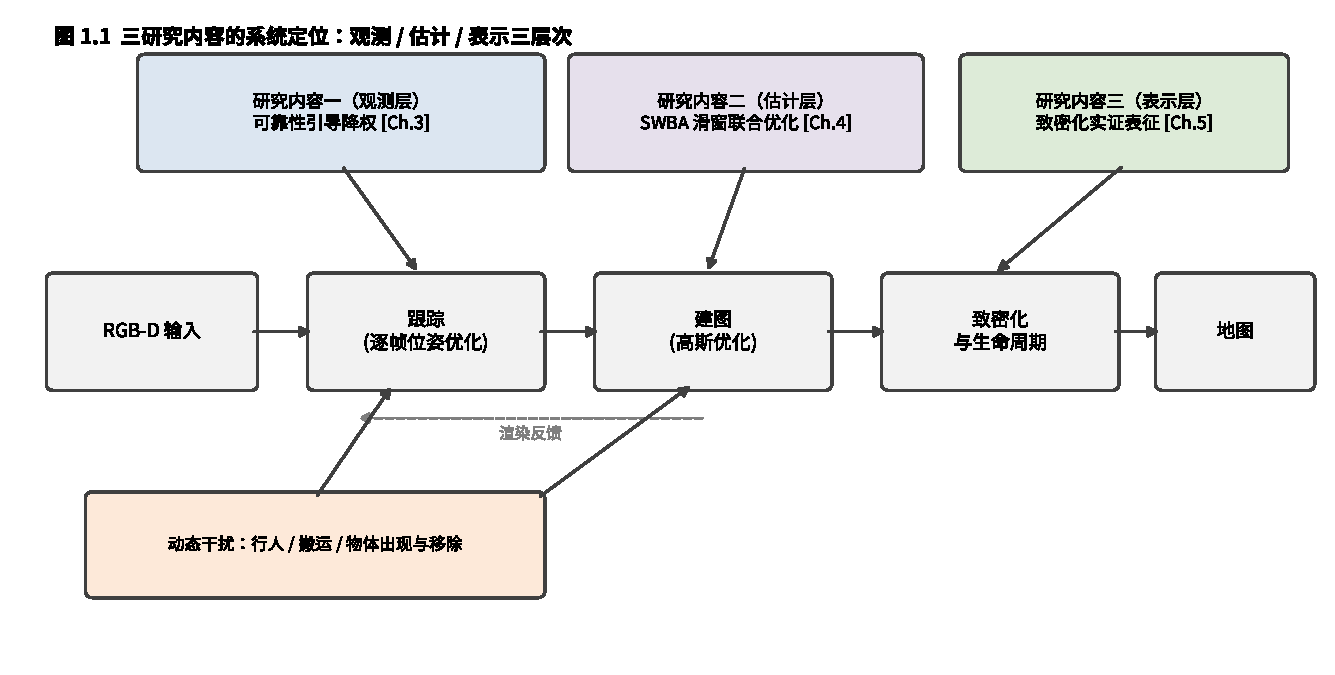
\includegraphics[width=0.95\textwidth]{figures/fig1_architecture.pdf}
  \caption{三研究内容的系统定位。观测层处理哪些像素可信，估计层处理位姿链的一致性，
    表示层处理地图基元的演化。三层沿 RGB-D 输入到地图的流水线依次承接，
    动态干扰自下而上进入跟踪与建图。}
  \label{fig:ch1-architecture}
\end{figure}

\section{论文组织结构}

全文共六章。第一章交代背景、现状、三个研究内容与组织结构。第二章给出相关工作，
沿致密化判据、动态高斯 SLAM、运行后地图的压缩与维护三条线展开。第三章对应研究内容一，
第四章对应研究内容二，第五章对应研究内容三。第六章总结全文并讨论后续方向。
各章数字的来源批次与序列集合在对应表脚注中逐项注明，口径不混引。

% chapters/ch2_related_work.tex — 第 2 章 相关工作
%
% ⚠ 待定：第 1 章已有「国内外研究现状」时，是否需要独立的相关工作章，
%    取决于三个研究内容各自相关的文献量。定稿前先决定，见 OUTLINE.md 的「待决问题」。
%    本节按「可独立成章、也可并入第 1 章现状节」的两用粒度写作。

\chapter{相关工作}
\label{ch:related}

\section{三维高斯的致密化判据}
\label{sec:related-densification}

3DGS 用一组各向异性的三维高斯表示场景，训练中靠自适应密度控制（adaptive density
control，ADC）决定地图的放大。原始判据很直接，把每个高斯在可观测视角上的屏幕空间
位置梯度取均值，跨过阈值就克隆或分裂，再按尺度与不透明度剔除退化基元。这个设计把
「该不该长」压缩成一个标量统计。统计口径本身没有区分梯度从哪种像素来。在线增量式
SLAM 里，MonoGS~\cite{MonoGS} 把这套 ADC 原样搬进关键帧循环，地图生长因此继承了它的
全部假设。

静态重建侧的工作很快发现，这个统计口径的每个环节都不是中性的管道。归一化一端，
Pixel-GS~\cite{pixelgs} 指出大高斯在多数视角只覆盖边缘少量像素，按视角简单取平均会把
高梯度摊薄，于是改按覆盖像素数加权。梯度方向一端，AbsGS~\cite{absgs} 把高频细节糊化
归因于梯度碰撞。大高斯在不同视角受到方向相反的位置梯度，均值永远低于阈值，该分裂的
不分裂，改用同向分量作判据。StopThePop~\cite{stopthepop} 从排序入手，分层逐像素重排
消除 popping，顺带发现视图一致性修复后所需高斯数约省一半。分母一端，Rogge
等~\cite{counting_contributions} 证明视锥可见性过滤对遮挡是盲的，被遮挡高斯照样计数，
摊薄信号、饿死遮挡区，于是把统计限制在实际贡献渲染的视角，并用平均贡献量替代原始
视角计数。信号形态一端，ACD-GS~\cite{acdgs} 认为一阶屏幕梯度分不清真实几何不连续与
高频纹理残差，改用二阶深度响应作曲率先验，并对克隆与分裂施加不对称调节。预算与调度
一端，Taming~3DGS~\cite{taming3dgs} 把无限增长改成逐像素光度贡献加权的构造式精确预算，
MCMC 视角~\cite{mcmcgs} 则把克隆与分裂整体改写为保概率的重定位，在固定基元数下完成
采样迁移。这些修正彼此独立，合起来指向同一个事实。致密化统计的口径会系统性地决定
高斯长在哪里，改动任何一个环节都能改变地图的形态。

动态场景给这条判据链补上了时间维度。RobustSplat~\cite{robustsplat} 在离线多视角设定
下指出，致密化过程本身会把瞬态扰动长进地图，动态物体存在越久，为它克隆出的高斯越多。
该方法先用延迟增长稳住静态结构，再做瞬态掩码自举。TAD-GS~\cite{tadgs} 进一步把时间
可见性直接写进判据。短寿命基元因监督稀疏而致密化不足，它按高斯的时间存在跨度调节
阈值。在线增量设定则是另一番情形。SLAM 系统只有因果观测，没有未来帧，MonoGS 一系的
工作大多沿用原版 ADC。更进一步的质疑来自 TopoGS-SLAM~\cite{topogsslam}，它在静态室内
基准上论证精度在中等基元数就趋于饱和，继续残差驱动地增长只是徒增显存，改用固定拓扑加
覆盖率触发的初始化，把建图变成有界维数的问题。离线一侧说动态区域需要时间感知的
致密化，在线静态一侧说致密化可能根本不必要，两个方向挤压着中间地带。在线动态场景里
的致密化决策，也就是观测因果、以跟踪误差为终点、逐事件控制注入量的那类决策，仍然
缺少专门的处理。这是第 5 章研究内容三的切入点。

\section{动态场景中的高斯 SLAM}
\label{sec:related-gs-slam}

把动态物体从轨迹估计里分出去，是动态 SLAM 的传统主线。DynaSLAM~\cite{DynaSLAM} 用语义
分割加多实例跟踪，把运动像素从数据关联中剔除，再对被遮挡的背景做补绘。这一类先掩蔽、
后重建的做法划定了后续十年的问题形态：动态区域不参与位姿估计，地图只描述静态世界。
它的代价也很明确，被剔除的区域不产生任何地图内容，掩码错了就一并抹掉真实结构。

高斯地图改变了这个格局。可微渲染让位姿、深度与地图进入同一个优化循环，SplaTAM~\cite{SplaTAM}
沿渲染误差优化相机，稠密地图随优化自然生长；DGS-SLAM~\cite{DGSSlam} 把高斯表示引入动态
环境，在剔除动态区域的同时保留完整地图。地图从被动产物变成了可优化的变量。新的问题也
随之而来，渲染误差对像素级扰动高度敏感，动态物体造成的光度残差若不处理，会同时污染
位姿和地图。WildGS-SLAM~\cite{wildgsslam} 为像素引入不确定性，让残差大的区域自动降权，
把「信多少」交给数据本身。本文作者此前的工作 RoGS-SLAM~\cite{RoGSSLAM} 沿同一条思路，
用光流一致性构造可靠性权重，在跟踪与建图中对动态观测降权而不做硬剔除，在 BONN 动态
序列上验证了这条可靠性路线的上界。这些工作的共同点是都在处理「观测是否可信」，即可靠
性信号作用在跟踪与优化的入口。

入口之后的环节少有人问。观测被加权或剔除之后，地图依然按静态规则生长，哪些高斯该
克隆、该分裂、该删除，仍然由致密化统计说了算，而这套统计对「像素为什么不可信」没有
概念。第 2.1 节的修正谱系处理的是统计口径本身的偏差，动态在线设定下还多出一层，统计
的输入就被动态残差污染。研究内容一管观测入口，研究内容二管运行后的地图维护~\cite{CompressionSurvey}，
中间的地图生长环节是第 5 章要补的位置。


% 三个研究内容，各占一章。⚠ 章节划分尚未定稿，见 03_main/OUTLINE.md。
% chapters/ch3_study1.tex — 第 3 章 研究内容一
%
% 对应小论文：MMM2027（RoGS-SLAM，camera-ready 14 页）
% 改写纪律：不直接翻译会议论文；claim 强度按大论文展开；实验数字须从
% results/evidence 工件重取（见 ../WRITING_RULES.md 六、七）。
% 本次只写 引言 + 方法；实验小节待数字核对后补，小结留骨架。

\chapter{动态场景下的可靠性引导观测处理}
\label{ch:study1}

\section{引言}

同步定位与地图构建（simultaneous localization and mapping，SLAM）在动态场景里
遇到的困难不在静态几何，而在观测本身不可信。行人走进视野，它在图像上的位移既可能是自身
运动，也可能是相机运动造成的视差；把两者混在一起交给跟踪器，位姿估计会被拖偏，
把两者一起当作噪声剔掉，又可能连带着删掉真实结构。动态 SLAM 的第一道关口因此不是
怎样建图，而是怎样判断一次观测该信多少。

早期做法沿着「先分割、后剔除」的路线展开。DynaSLAM~\cite{DynaSLAM} 用语义分割与
多实例跟踪圈出运动像素，直接从数据关联中去掉，再对被遮挡的背景做补绘。这条路线
简单有效，代价是把观测当成二值开关，一旦掩码出错，真实结构也一并被抹掉。语义分割
在两类场景下格外脆弱，一是物体运动但语义上不属于「动态类」的情形，二是分割模型
没有见过的场景，这两类失败在野外数据里都不罕见。

另一种思路是保留观测，只调整它的权重。既然错误的观测会持续给出与几何不一致的残差，
那么就用残差本身判断可信度，让可疑的观测平滑降权而不是骤然删除。研究内容一沿这条
思路，回答第 1 章提出的问题，即哪些观测可以进入跟踪和建图。本章的方法由四个组件
组成，合起来把「信多少」落成逐像素、逐帧的可计算量。

\section{方法}
\label{sec:study1-method}

\subsection{可靠性信号}

可靠性信号的核心是构造两个可以互相校验的流量。观测流来自图像上相邻关键帧之间的
像素位移，由光流给出；刚体流则把上一帧的深度反投影到世界坐标，再用当前位姿投回
图像平面，得到如果场景完全静止时像素应该出现的位置。两者之差衡量的是「观测不符合
刚体假设」的程度。场景里的移动物体、未被建模的形变、深度噪声都会抬高这个残差，
被遮挡后重新露出的区域同样如此。

残差本身不能直接当权重用。行人在视野边缘时残差会短暂升高，人物静止不动时残差
接近零，单帧的读数波动很大。方法把逐像素残差转成 Cauchy 分布的似然，用来做只降不升
的重加权。Cauchy 的尾部比高斯厚，允许少数极大的残差被当作离群点压下去而不影响
大部分像素的权重；只降不升保证可靠性信号永远不会把本已可疑的观测抬得比原始观测更高，
避免信号自身的错误被放大成增益。

\subsection{鲁棒重加权}

跟踪环节的残差用 Huber 损失做迭代重加权。Huber 在残差较小时保持二次型，残差较大时
切换为线性，从而限制单次更新的影响力。这一步与可靠性信号互补，后者处理「像素是否
符合刚体假设」，前者处理「位姿更新是否被少数大残差带偏」。两者都作用在跟踪的入口，
不触碰建图端的高斯表示。

\subsection{关键帧覆盖}

关键帧的选取在人群场景里容易被运动物体带偏。行人经过时画面变化剧烈，按常规的图像
差异准则会连续插入关键帧，结果是关键帧密集堆在同一个视野，重建却缺少长程覆盖。
方法改用统一的覆盖准则，让关键帧分布服从场景几何而不是局部图像差异，同时限制相邻
关键帧的间隔上限，避免长距离漂移无人校正。

\subsection{lineage 生命周期}

第四个组件处理高斯的来去。运动物体在视野里停留的时段内，会有一批高斯被临时创建
来拟合它；物体离开后，这些高斯没有观测支撑，却可能因为不透明度尚未衰减而残留在
地图里。方法给每个高斯记录来源与代际，把「何时可以提交、何时应当回收」变成可审计的
生命周期，而不是依赖统一的不透明度阈值。语义掩码作为可选组件保留，与可靠性信号
叠加使用，不单独承担判断。

四个组件的共同点是把动态观测当作概率对象处理：不判断它是否动态，只估计它有多可信；
不一次性删除，而是持续降权并记录来源。第 3.3 节报告这些组件在标准动态序列上的
效果与边界，数字的工件来源见各表脚注。

% TODO(写作队列)：3.3 实验（数字须从 RoGS-SLAM/results/evidence 重取并与表逐格核对）；
% 3.4 小结（按 WRITING_RULES 四，避免复述式小结，写边界与适用条件）。

% chapters/ch4_study2.tex — 第 4 章 研究内容二
%
% 对应小论文：CVM2027（动态场景高斯地图的解剖、压缩与离线修复，在投）
% 改写纪律：不直接翻译会议论文；实验数字须从 RoGS-Map/results 与
% monogs-ours/results 工件重取并核口径（WRITING_RULES 六、七）。
% 本次写 引言 + 方法（三小节）；实验与小结留写作队列。

\chapter{动态场景高斯地图的表示、压缩与离线修复}
\label{ch:study2}

\section{引言}

第 3 章处理的是观测进入系统的入口，本章换一个对象：系统跑完之后留下的那张地图。
动态场景的高斯地图有两个与静态场景不同的性质。第一，它同时包含静态结构与大量为
动态物体临时创建、随后失去观测支撑的基元，这些基元的外观与几何都不符合任何真实
表面。第二，它的规模随轨迹长度增长，而在动态场景里增长的相当一部分来自这些临时
基元。前者影响地图能不能被继续使用，后者影响地图能不能被存下来。

已有工作大多把动态处理放在运行期。第 3 章的方法在跟踪入口给观测降权，DynaGSLAM
一类的工作则在建图期把动态物体建成独立的层，靠可见性管理它们的生命周期。两条
路线共同的隐含前提是动态内容在运行期就可以判断清楚。实际情况是，运行期的判断依赖
当时可见的证据，一个物体在离开视野后被误判、或者静止期间被漏判，错误就会沉淀进
地图，事后没有人再纠正它。研究内容二因此把地图当作研究对象，回答三个问题。一张动态场景的高斯地图贵在哪里、
差在哪里，它能不能被高效压缩，被反动态范式抹掉的动态内容能不能在离线阶段装回去。

\section{方法}
\label{sec:study2-method}

\subsection{地图解剖与代价刻画}

要回答「贵在哪里」，先要有一张可比的底图。方法从 11 个可复现的 SLAM 系统出发，在同一
批动态序列上产出地图，用同一套指标横比，从而把「系统差异」与「动态内容本身的开销」
分开。指标沿三条线展开：基元数量与显存占用衡量规模，静态区与腾空区的渲染质量衡量
代价，几何指标（深度 L1）与外观指标（PSNR）分开报告以区分「几何错了」与「贴图错了」。

腾空区是这项分析的核心对象。它最贵。反动态范式把动态物体从地图中剔除，物体离开后原本被它
占据的空间既没有观测也没有基元，渲染时只能由周围基元外推，于是出现明显的劣化。
方法把腾空区单独切片测量，并做两项拆解。一是按基元尺度与不透明度分组，看劣化由哪类
基元承担；二是把误差按深度分层，排除「只是近处像素多」这类构型偏差。这两项拆解
在后续的修复算子里直接决定应该往哪里补基元。

\subsection{离线地图压缩}

压缩的对象是已经冻结的地图，因此可以用比训练期更激进的策略。方法沿三条线做无损到有损的连续调节。属性量化把位置、尺度、旋转、球谐系数与不透明度
分通道量化，各通道的比特预算按贡献度分配；剪枝按「删除后渲染误差最小」排序，逐图
自适应地删到预算；熵编码对量化后的残差做上下文建模。三条线合起来，同一张地图可以按需求在近无损到
激进压缩之间选择工作点，压缩率与渲染质量的权衡由曲线给出而不是单一数字。

这条路线与训练期压缩的区别值得说明。训练期压缩要参与梯度回传，因此只能用可微的
近似；离线压缩没有这个约束，可以把熵模型做得更紧，也可以做全局的重排序。代价是
它必须假定地图不再变化，这一假定与第 5 章关注的地图在线生长是互斥的，两章的结论
不能直接相互引用。

\subsection{离线动态修复}

修复要解决的是第 4.2 节测出来的那个洞。方法把 DynaGSLAM 式的动态高斯管理从运行期
搬到离线：修的是已冻结的地图，静态层的每一个基元在修复前后逐位不变，只有腾空区
内部按观测重建。离线修复切断了这条环路。运行期修复会改变跟踪所依赖的地图，误差会通过
跟踪环路反馈回位姿；代价是修复只能作用于已经建好的地图。

修复算子本身的形态是逐区域的两阶段。先在腾空区内部用多视角一致性挑出可靠的深度观测，
再按观测到的表面补一组新基元并做局部优化。优化的目标函数只包含静态层与
新基元的渲染一致性，不触碰原始地图。评价沿用第 4.2 节的三条线，并额外报告一个问题。修复后的地图在多大程度上仍可被视为
「同一张地图」，也就是静态层不变的约束有多强。

三项工作共同把地图从「系统输出的副产品」变成「可以独立分析、压缩与修复的对象」。
第 4.4 节报告这批读数与边界，数字的工件来源见各表脚注。

% TODO(写作队列)：4.4 实验（数字从 RoGS-Map/results/evidence 与 monogs-ours results 重取，
% 注明批次与序列集合；与第 3 章的序列集合差异要写明）；4.5 小结（写边界，不复述）。

% ============ 4.3 实验 + 4.4 小结（2026-11-08 成文；关卡② 待审） ============
% 数字来源纪律：全部数字出自 CVM2027 投稿件批次。表 4.1~4.4 行由 RoGS-Map/papers/
% paper2/tables/*.tex 程序化提取（生成器脚本可复跑，"do not edit by hand" 工件），
% 全部 239 处数字经 RoGS-Map/PROVENANCE 逐格核验命中。retention 拆解出自
% monogs-ours/results/paper2_fulltable/evidence/dyn_cost_decomp_2026-10-05.md。
% 红线（R2_sections/07）：修复机制本体归 DynaGSLAM 必引；在线↔离线禁混引（J3 性质
% 相反分开表述）；禁"首个恢复动态"；codec 联动未做不声称。

\section{实验}
\label{sec:study2-exp}

\subsection{实验底图与协议}

地图研究的全部读数都长在底图上，底图本身要先交代。本章的底图由第 3 章的先验 RGB-D
栈在 BONN 动态序列上运行产生，其跟踪质量见表~\ref{tab:study2-baseline}：六条公共
序列上 2.2 到 5.5 厘米，两条 person\_tracking 为 11.3 与 10.4 厘米。表中的 11 个
复现系统与本栈同机同协议评测，静态方法在动态序列上严重退化，动态方法分布在 1.6 到
20 厘米之间。先验栈一行在本章只作背景，它是地图研究的出发点，不是本章的结果。

\begin{table}[htbp]
\centering
\footnotesize
\setlength{\tabcolsep}{3pt}
\caption{公共 BONN 序列上的绝对轨迹误差（RMSE，厘米，3 种子均值±标准差，全轨迹
Horn SE(3) 对齐；上排 11 系统为同一台机器的复现，DynaGSLAM 委托外部前端定位故无
方差；上标 d 表示首次运行发散、按协议重跑后的取值；末行为论文一的先验栈，独立批次
同机同协议，作本章背景）}
\label{tab:study2-baseline}
\begin{tabular}{@{}llcccccc@{}}
\toprule
方法 & 表示族 & balloon & balloon2 & crowd & crowd2 & person\_tracking & person\_tracking2 \\
\midrule
\multicolumn{8}{@{}l}{静态方法} \\
MonoGS~\cite{MonoGS} & 3DGS & 39.32$\pm$1.01 & 22.05$\pm$1.55 & 86.47$\pm$18.34$^\mathrm{d}$ & 147.46$\pm$39.03$^\mathrm{d}$ & 44.83$\pm$9.06 & 43.85$\pm$8.55 \\
SplaTAM~\cite{SplaTAM} & 3DGS & 36.50$\pm$0.53 & 37.47$\pm$2.87 & 135.37$\pm$36.15$^\mathrm{d}$ & 493.22$\pm$470.66$^\mathrm{d}$ & 92.52$\pm$18.93$^\mathrm{d}$ & 132.72$\pm$9.37$^\mathrm{d}$ \\
Co-SLAM~\cite{CoSLAM} & implicit & 27.10$\pm$0.97 & 35.10$\pm$4.07 & 35866.32$\pm$38265.29$^\mathrm{d}$ & 24905.40$\pm$42817.31$^\mathrm{d}$ & 75.50$\pm$6.52 & 71.26$\pm$2.90 \\
ORB-SLAM3~\cite{ORBSLAM3} & classical & 7.27$\pm$1.45 & 19.81$\pm$2.18 & 76.60$\pm$27.86$^\mathrm{d}$ & 111.41$\pm$14.75$^\mathrm{d}$ & 69.54$\pm$2.19 & 76.82$\pm$2.14 \\
\midrule
\multicolumn{8}{@{}l}{动态方法} \\
DG-SLAM~\cite{dgslam} & 3DGS & 3.66$\pm$0.02 & 3.83$\pm$0.08 & 5.76$\pm$0.15 & 6.39$\pm$0.50 & 4.25$\pm$0.06 & 6.12$\pm$0.13 \\
RGD-SLAM~\cite{RGDSLAM} & 3DGS & 2.45$\pm$0.22 & 4.26$\pm$0.89 & 2.61$\pm$0.28 & 2.36$\pm$0.06 & 7.21$\pm$1.24 & 20.10$\pm$2.55 \\
WildGS-SLAM~\cite{WildGS} & 3DGS & 2.75$\pm$0.07 & 2.42$\pm$0.04 & 1.55$\pm$0.06 & 2.17$\pm$0.05 & 3.63$\pm$0.08 & 3.09$\pm$0.03 \\
DynaGSLAM~\cite{dynagslam} & 3DGS & 8.36 & 9.36 & 23.82 & 13.73 & 8.94 & 13.69 \\
DynaSLAM~\cite{DynaSLAM} & classical & 2.88$\pm$0.16 & 2.59$\pm$0.10 & 2.07$\pm$0.21 & 2.85$\pm$0.28$^\mathrm{d}$ & 4.53$\pm$1.81 & 8.82$\pm$1.18 \\
NGD-SLAM~\cite{NGDSLAM} & classical & 2.82$\pm$0.07 & 2.46$\pm$0.08 & 1.85$\pm$0.16 & 2.22$\pm$0.07 & 4.97$\pm$0.44 & 6.63$\pm$0.43 \\
RoDyn-SLAM~\cite{rodynslam} & implicit & 8.47$\pm$0.31 & 11.90$\pm$0.21 & 5.60$\pm$0.18 & 4.63$\pm$0.06 & 16.39$\pm$0.54 & 14.36$\pm$0.11 \\
\midrule
先验 RGB-D 栈（论文一）& 3DGS & 3.25$\pm$0.07 & 5.48$\pm$0.27 & 2.23$\pm$0.10 & 2.26$\pm$0.32 & 11.31$\pm$0.70 & 10.40$\pm$0.28 \\
\bottomrule
\end{tabular}
\end{table}

\subsection{地图的字节构成}

一条 SH 零阶的高斯基元占 80 字节，栅格化器只读其中 14 个字段共 56 字节，其余 6 个
字段 24 字节是渲染器从不读取的记账信息，占原始字节的 30\%。把熵编码从 14 个渲染字段
扩到全部 20 个字段，码率只多付 1.04 倍。这两条读数合起来说明，对 SLAM 地图做朴素的
字节级压缩，首先被压掉的部分里有接近三成是与画面无关的簿记，字节预算的字面数字
高估了地图的实际内容。

几何统计给出第二个观察。测过的 14 张动态地图里，88.8\% 到 94.7\% 的四元数偏离
单位范数超过 1\%，旋转参数存在普遍的冗余自由度。动态地图中 78\% 到 92\% 的基元
接近各向同性，干净的静态序列里这个比例只有 52\% 到 76\%，有人走动时升到 81\% 到
85\%，坐姿人群高到 89\% 到 91\%。动态内容倾向于把基元推向各向同性，这为后面按
尺度分组的压缩策略提供了直接的统计依据。
% 来源：paper2_cvm.tex §4（gate2 注记：storage_census_2026-10-05.md、anatomy_census.json、
% l1_readout_2026-10-04.md）。

\subsection{压缩率与质量的工作点}

表~\ref{tab:study2-rd} 给出七条 Bonn 序列、三种子平均的压缩率与质量曲线。
无损层里通用压缩器只能拿到 1.37 到 1.62 倍。有损层里两个后训练学习基线把压缩率推到
6 倍以上：SOG 量化后 6.53 倍、全图 PSNR 只掉 0.02 分贝；Niedermayr c3dgs 用量化感知
训练重拟合 5 千步，6.15 倍且全图 PSNR 反升 0.77 分贝，代价是必须逐图重新训练。
本方法的三个工作点不做任何重训练：近无损点 5.96 倍、全图只掉 0.01 分贝；中间点
8.77 倍、掉 0.06 分贝，落在质量与码率的最优带；激进点 15.11 倍、全图掉 0.64 分贝，
静态区掉约 2.7 分贝，held-out 序列上外推最差（负 1.77 分贝），如实报告。
% 来源：tab_rd（scripts/gs_compress/paper2_codec_tables.py 生成；D2-025 L1/L2/L3 +
% post-hoc generic + learned baselines 批次）。

\begin{table}[htbp]
\centering
\footnotesize
\setlength{\tabcolsep}{3pt}
\caption{七条 Bonn 序列上的压缩率与质量（三种子均值；量化位宽按位置/不透明度/
缩放/旋转/球谐顺序；held-out 为未参与调参序列的静态 PSNR 变化）}
\label{tab:study2-rd}
\begin{tabular}{@{}lcccrccr@{}}
\toprule
方法 & 量化位宽 & 压缩率 & 字节/基元 & 全图 PSNR & $\Delta$ & 静态 PSNR & held-out $\Delta$ \\
\midrule
\multicolumn{8}{@{}l}{源文件与无损通用压缩器} \\
\quad source (uncompressed, 20-field f32) & -- & 1.00$\times$ & 80 & 15.38 & $0.00$ & 21.95 & $0.00$ \\
\quad zlib (lossless) & -- & 1.47$\times$ & 54.3 & 15.38 & $0.00$ & 21.95 & $0.00$ \\
\quad zstd (lossless) & -- & 1.54$\times$ & 51.8 & 15.38 & $0.00$ & 21.95 & $0.00$ \\
\quad lzma (lossless) & -- & 1.62$\times$ & 49.3 & 15.38 & $0.00$ & 21.95 & $0.00$ \\
\quad blosc2 (shuffle+delta) (lossless) & -- & 1.37$\times$ & 58.2 & 15.38 & $0.00$ & 21.95 & $0.00$ \\
\midrule
\multicolumn{8}{@{}l}{有损基线（通用截断与后训练学习）} \\
\quad blosc2 TRUNC\_PREC=16 (lossy) & -- & 2.84$\times$ & 28.1 & -- & -- & -- & -- \\
\quad blosc2 TRUNC\_PREC=8 (lossy) & -- & 3.80$\times$ & 21.1 & -- & -- & -- & -- \\
\quad SOG~\cite{SOG} & -- & 6.53$\times$ & 12.2 & 15.36 & $-0.02$ & 21.82 & $-0.04$ \\
\quad Niedermayr c3dgs~\cite{Compressed3DGS} & -- & 6.15$\times$ & 13.0 & 16.15 & $+0.77$ & 20.94 & $-0.01$ \\
\midrule
\multicolumn{8}{@{}l}{本文（均匀量化 + zlib 编解码，有损）} \\
\quad near-lossless & 16/8/8/8/8 & 5.96$\times$ & 13.4 & 15.37 & $-0.01$ & 21.79 & $-0.00$ \\
\quad mid & 10/6/6/6/6 & 8.77$\times$ & 9.1 & 15.32 & $-0.06$ & 21.64 & $-0.21$ \\
\quad aggressive & 8/4/4/4/4 & 15.11$\times$ & 5.3 & 14.74 & $-0.64$ & 19.21 & $-1.77$ \\
\midrule
\multicolumn{8}{@{}l}{消融：加体素合并（非工作点）} \\
\quad near-lossless + voxel merge & 16/8/8/8/8 & 7.81$\times$ & 10.2 & 15.30 & $-0.08$ & -- & -- \\
\quad mid + voxel merge & 10/6/6/6/6 & 11.26$\times$ & 7.1 & 15.25 & $-0.13$ & -- & -- \\
\quad aggressive + voxel merge & 8/4/4/4/4 & 19.00$\times$ & 4.2 & 14.72 & $-0.66$ & -- & -- \\
\bottomrule
\end{tabular}
\end{table}

\subsection{反动态代价}

表~\ref{tab:study2-dyncost} 测量反动态政策的代价：把被抹掉的动态内容原样插回冻结
地图，量的是天花板，不是任何在线系统的达成值。五条序列的动态区增益 17.9 到 22.2
分贝，同区深度误差比 0.16 到 0.27，全图增益 5.4 到 12.0 分贝；静态区没有一条受损，
变化全部为正。代价与拥挤度正相关，人群序列最高，跨序列在 6\% 到 29\% 之间，中位
22\%。

\begin{table}[htbp]
\centering
\small
\caption{反动态代价的逐序列读数（冻结地图插入探针，canonical 掩码分区；动态区 =
真实损坏子集；每序列两图取基线臂）}
\label{tab:study2-dyncost}
\begin{tabular}{lcccc}
\toprule
序列 & 动态区增益 & 动态区深度比 & 全图 & 静态区 \\
 & (dB) & （越低越好） & (dB) & (dB) \\
\midrule
crowd & 22.2 & 0.19 & +12.0 & +0.29 \\
crowd2 & 21.6 & 0.18 & +10.6 & +0.04 \\
crowd3 & 21.0 & 0.19 & +10.4 & +0.39 \\
person\_tracking & 19.5 & 0.27 & +8.7 & +0.28 \\
balloon2 & 17.9 & 0.16 & +5.4 & +0.33 \\
\bottomrule
\end{tabular}
\end{table}

几何与外观的拆解回答代价由什么承担。把插入的动态基元按有无运动分组，无运动组的
基元保留率 0.80 到 0.93，冻结组只有 0.10 到 0.39。被抹除区域的大半渲染质量其实
靠把动态几何留在地图里挽回，逐帧运动本身不是主要杠杆。在线阶段如何以可负担的方式
达成这一天花板，属于第 5 章的在线生长问题，两章口径互斥。
% 来源：tab_dyncost_seq（dyn_cost_5seq_2026-10-05.json）+ dyn_cost_decomp_2026-10-05.md
%（retention 拆解）+ verdict_dyn_cost_5seq（成本 6–29%，中位 22%）。

\subsection{离线修复}

修复算子把 DynaGSLAM~\cite{dynagslam} 的动态高斯管理从运行期搬到离线：修的是已冻结
的地图，静态层逐位不动，只有腾空区按观测重建。表~\ref{tab:study2-dynport} 把同一
机制的两种放置放在同一张表里。离线是完整的七序列、三种子网格，21 格全部通过预注册
门：动态区增益 5.49 到 8.95 分贝，深度比 0.23 到 0.61，静态区变化在负 0.035 到
正 0.196 分贝之间，即静态层确实逐位未动。

\begin{table}[htbp]
\centering
\small
\caption{同一动态高斯管理的在线与离线放置对照（对照基线 = 抹除；在线代价为逐帧建图
开销增幅，离线代价为修复占底图在线墙钟的份额；离线为 7 序列 × 3 种子全网格 21 格，
在线仅两序列；该对照为描述性而非单变量，见正文）}
\label{tab:study2-dynport}
\begin{tabular}{@{}lccccc@{}}
\toprule
放置 & 动态区增益 J1 (dB) & 深度比 J2 & 静态区 J3 (dB) & 代价 & 结果 \\
\midrule
在线（同一机制）& $+6.97/+6.96$ & 0.35/0.26 & $-0.49/-1.02$ & $+95.1/+88.6\%$ & fail \\
抹除（参照）& $0$ & $1$ & $0$ & --- & --- \\
离线（本文）& $+5.49$--$+8.95$ & 0.23--0.61 & $-0.035$ to $+0.196$ & 0.11--0.30$\times$ & pass 21/21 \\
\bottomrule
\end{tabular}
\end{table}

同一机制在线运行的对照行需要两句限定。其一，把机制从在线搬到离线同时改变了位姿
来源、静态层保护、关键帧日程与掩码通路四件事，这一对照描述的是放置选择的总效应，
不是单变量归因。其二，在线两序列的动态区读数来自快照口径仪器，位姿与被评帧不同源，
含位姿混杂，与离线数字不可比；两行的静态区指标性质也不同，离线是逐位未动，在线是
联合优化中被改。

输出形态是设计决策而不是局限。单 PLY 合并形态正是动态内容丢失的形态，把动态内容
装回去必须以层序列保存，静态层才能保持逐位不变。压缩编解码只能消费层序列输出，
不能消费合并后的单文件，两者的联动不在本章范围内。
% 来源：tab_dynport（offline = results/dynport_offline/evidence_L3 manifest；
% online = results/dynport/evidence/manifest_L1_v2.json，snapshot 口径）。

\section{小结}
\label{sec:study2-summary}

本章回答引言提出的四个问题。贵在哪里：80 字节的基元里三成是渲染器不读的记账字段，
四元数与各向同性统计给出压缩的统计着力点。差在哪里：反动态范式抹掉的动态内容在
冻结地图上值 17.9 到 22.2 分贝的动态区增益，代价与人群密度正相关，且大半由几何
保留而非外观优化承担。能不能压缩：不重训练的三个工作点覆盖 6 到 15 倍，中间点
8.77 倍只掉 0.06 分贝，学习型基线的强读数以逐图重训练为前提。能不能装回：离线
放置的动态管理 21 格全部过门，静态层逐位未动，同一机制在线因开销不可负担。

边界与适用条件：压缩的激进点在 held-out 序列上外推最差；修复以层序列为输出形态，
与单文件压缩不联动；在线与离线读数来自不同仪器口径，本章不混引。全部数字出自
CVM2027 投稿件批次，工件经 239 处逐格核验。
% WRITING_RULES 四：小结不复述表格细节，只留四问四答与边界。

% chapters/ch5_study3.tex — 第 5 章 研究内容三
%
% 研究内容三：动态场景高斯地图的时间感知致密化（实证表征）。
% 章标题沿 OUTLINE 第四章结构定名；内容按 2026-11-07 用户拍板的「戊·两步走」
% 重定向为实证表征（monogs-ours paper3/ 一页纸 onepager_wu_boundary_2026-11-07 §一）。
%
% 数字来源纪律（WORKFLOW 铁律 2 数字零手抄 + WRITING_RULES 六）：
% 全部实验数字出自 monogs-ours/paper3/results/evidence/ 的判决文档与 judge JSON，
% 各节以 % 注释给出来源指针；剂量过供给第三 seed 补批（Amendment A1）与 async
% 迁移检查（P3-D2-043）收口后相关数字随之刷新（2026-11-08 派发中）。
% 测量口径红线：仪器口径（单线程+确定性栅格化）读数与 async 部署口径读数
% 永不混引，绝对 ATE 不跨口径、不跨机并列。

\chapter{动态场景高斯地图的时间感知致密化}
\label{ch:study3}

\section{引言}

第 3 章处理的是观测进入系统的入口，第 4 章处理的是系统跑完之后留下的地图。本章回到
两者之间那个持续发生的环节：地图的生长。在线高斯 SLAM 的地图不是一次建成的，系统每
隔一段迭代就执行一次致密化检查，把梯度大的点一分为二或克隆一份，让地图跟着观测逐步
长出几何支撑。这套机制继承自静态场景的三维高斯泼溅，在动态场景里它面对的问题是同一个吗，
默认参数还需要外部干预吗，干预的收益由什么决定，这三个问题构成本章的研究对象。
% 来源：paper3/PROBLEM.md §1-2（研究问题）；章节边界句沿 ch3/ch4 入口-地图-生长的组织线
% （OUTLINE.md §二 Q2：可靠观测 → 地图表示与维护 → 地图生长）。

对这三个问题，本章的回答是一份实证表征。选择轴上，我们系统测试了五类外置干预机制，
包括按统计纯度加权、按观测次数设资格门、按未命中计数加剪枝、以及两种剂量调整，
没有一类产生净收益，管线自带的剪枝自调节承担了原本指望干预承担的职能。剂量轴上，
测量给出从完全关闭到四倍阈值的三测点前沿，完全关闭使跟踪误差恶化三点六厘米、
地图缩到原来的百分之十五，说明致密化是明确的正资产，同时默认剂量也不在前沿的
最低点。序列之间，同样的减量干预在人群序列回收零点七厘米，在移动箱体序列反而
有害，收益方向不由场景的动态占比预测。这些读数合起来给出一个可操作的判据，
告诉后来者在什么条件下不必再设计此类机制，也把算力指向真正有杠杆的地方。
% 来源：onepager_wu_boundary_2026-11-07 §一（主张，2026-11-07 按泛化探针收窄）；
% 判决链 dose_a4_instrument / dose_scan / dose_oversupply（2026-11-06~08）。
% 注：正文中数字为骨架期锚定值，第三 seed 补批收口后刷新（Amendment A1，2026-11-08）。

\section{致密化机理与默认行为}
\label{sec:study3-mechanism}

理解干预为什么无效，先要看清管线在没有干预时做了什么。系统每积累一百次迭代就执行
一轮致密化检查：先按位置梯度挑出一批候选点，符合条件的高斯被克隆或分裂，使地图在
欠支撑的区域加出新的基元；随后按不透明度做一轮剪枝，把长期得不到观测支撑的基元
直接删除。clone 与 split 的触发由一个梯度阈值控制，阈值越低、每轮长出的基元越多，
这就是本文所说的剂量。剪枝不设阈值，凡不透明度衰减到下限以下的基元一律删除，
它是管线自带的清除机制。
% 来源：slam_backend.py densify_and_prune 调用点与 combined_prune/method.yaml
% 默认参数（densify_grad_threshold 0.0002、percent_dense 0.01、每 100 iter 执行）；
% 机理描述与 paper3/PROBLEM.md §1 一致。

这套默认行为里最关键的事实是剪枝自调节的强度。对一个生长中的地图连续记账的结果是，
致密化累计新增的基元里只有不到两成会被剪枝删除，其余都存活下来成为地图的长期成员；
换句话说，管线并非无节制地生长，无支撑的基元在出生后一两个检查周期内就会消亡。
这解释了后续各节一个反复出现的现象：外置干预试图替管线决定在哪里长、长多少，
而管线自身的选择与清除机制已经承担了大部分职能，干预要产生净收益就必须先超过
这个本底。
% 来源：paper3/results/evidence/growth_waste_balance_2026-11-06.md（prune÷新增 =
% 16.7%，83% 新生基元存活，40 帧仪器口径账本）；PROBLEM.md H1/H2 在本管线未获支持的
% 四条独立证据链之第一条（P3-D2-036）。

\section{测量方法}
\label{sec:study3-instrument}

本章的结论大多以零点几厘米的效应量出现，而跟踪误差本身就有厘米级的波动，测量装置
因此成为第一个要解决的问题。默认部署配置里有两个与设备无关的不确定性来源。其一是
异步调度，前端与后端各自推进，后端在两次关键帧之间跑多少次优化由墙钟决定，同样的
配置两次运行会走出不同的迭代数；其二是栅格化反向传播里的跨像素原子加法，浮点加法
的顺序不确定，梯度带着微小差异进入后续每一步。两者叠加的实测后果是，同一配置同一
随机种子重跑一次，跟踪误差可以相差两厘米以上，地图规模可以差出近一倍。
% 来源：device_floor_3090_2026-11-05.md（同 config 同 seed 重跑 online 极差 +96.8%，
% ATE 自差最高 2.14cm）；detraster_residual_bisect_2026-11-05.md（async 自由跑为
% 设备无关分叉源，同 20 帧两跑 735 vs 700 个不同 iteration）；P3-D2-022~026 装置诊断链。

测量方法把这两个来源逐个关闭。栅格化反向传播的浮点原子加法改写为整数镜像累加，
加法顺序不再影响结果；前端与后端都切到单线程固定步长，迭代数不再依赖墙钟；在此
之上叠加数值确定性套件。关闭之后，同一配置同一随机种子的两次运行在全部判据文件上
逐位一致，这一性质称为仪器有效性，作为每个正式批的前置门，两次运行有任何一位
不同则整批作废。这把装置的自差从厘米级压到零，使零点五厘米级的机制效应第一次
可以与噪声区分。
% 来源：prereg_instrument_mode_2026-11-05.md（三项锁定开关 + 三环境 + R-valid 判据）；
% detraster_L2_2x2_2026-11-05.md（2×2 四格，仅「单线程 × det-ON」达逐位一致）。

仪器口径与部署口径是两把不同的尺子，读数不能混用。单线程关闭了后端持续优化带来的
地图新鲜度，两者的跟踪误差与地图规模系统性地不同，本章所有臂级比较都在仪器口径内
完成；部署口径下的对应表现单列检验，两套读数分别登记，绝对值不与文献表格并列。
测量方法本身是使本章结论可判的前提，属于配套与评测卫生，不作为贡献主张。
% 来源：prereg_instrument_mode §0「它不是部署配置」（ATE 1.168 vs async 1.177、
% 高斯 19771 vs 25976）；DISCIPLINE「测量口径」#3 口径单源化 + 论文叙事纪律
%（评测协议不进贡献栏，用户 2026-09-25 裁定）。




% chapters/ch6_conclusion.tex — 结论与展望
%
% ⚠ 不要写成三章小结的拼接。结论要回答的是「这些工作合起来说明什么」，
%    不是「第三章说了什么、第四章说了什么」。具体做法见 WRITING_RULES.md 第四节。

\chapter{结论与展望}
\label{ch:conclusion}

\section{主要结论}

\section{研究局限}

\section{未来工作}


% ---------------------------------------------------------------- 后置部分
% frontmatter/bibliography.tex — 参考文献
%
% 用 bibtex + gbt7714 样式（国标 GB/T 7714-2015，中文论文通行）。
% 文献库在 refs/references.bib，两篇小论文的 bib 合并进来即可。
%
% 若学校要求著录格式与 gbt7714 有出入，改 refs/ 里的 .bst 或换 biblatex，
% 不要手工排参考文献列表。

\clearpage
\phantomsection
\addcontentsline{toc}{chapter}{参考文献}
\markboth{参考文献}{参考文献}

\begin{center}
{\heiti\zihao{3} 参考文献}
\end{center}
\vspace{1\baselineskip}

\begingroup
\zihao{5}
\setlength{\parindent}{2em}
\bibliographystyle{refs/gbt7714-numeric}
\bibliography{refs/references}
\endgroup

% frontmatter/acknowledgement.tex — 致谢
%
% 格式：标题三号黑体，两字中间空两格，居中；内容宋体小四，1.5 倍行距。
%
% 这一节必须本人写，AI 不代笔（见 WRITING_RULES.md 第十一节）。
% 这里只留位置。

\clearpage
\phantomsection
\addcontentsline{toc}{chapter}{致\quad 谢}
\markboth{致谢}{致谢}

\begin{center}
{\heiti\zihao{3} 致\quad 谢}
\end{center}
\vspace{1\baselineskip}

% TODO(本人写)

% frontmatter/appendix.tex — 附录
%
% 官方模板附录包含三部分：
%   一、在校期间发表的科研成果
%   二、在校期间参加的项目
%   三、在校期间获奖情况
%
% 发表成果的格式同参考文献，其他同正文（五号，无缩进，单倍行距）。

\clearpage
\phantomsection
\addcontentsline{toc}{chapter}{附\quad 录}
\markboth{附录}{附录}

\begin{center}
{\heiti\zihao{3} 附\quad 录}
\end{center}
\vspace{1\baselineskip}

\noindent{\heiti\zihao{4} 一、在校期间发表的科研成果}
\vspace{0.5\baselineskip}

\begingroup
\zihao{5}
\setlength{\parindent}{0em}
\begin{enumerate}
  \item 陈彬，苏洁. RoGS-SLAM: Robust Gaussian Splatting SLAM in Dynamic Environments
        via Reliability-Guided Weighting. MMM 2027（已录用）.
  \item 陈彬，苏洁. A Dynamic-Scene Gaussian SLAM Map: Anatomy, Compression, and
        Offline Repair. CVM 2027（已投稿）.
\end{enumerate}
\endgroup

\vspace{\baselineskip}
\noindent{\heiti\zihao{4} 二、在校期间参加的项目}
\vspace{0.5\baselineskip}

\begingroup
\zihao{5}\setlength{\parindent}{0em}
% TODO(本人填)
\endgroup

\vspace{\baselineskip}
\noindent{\heiti\zihao{4} 三、在校期间获奖情况}
\vspace{0.5\baselineskip}

\begingroup
\zihao{5}\setlength{\parindent}{0em}
% TODO(本人填)
\endgroup


\end{document}
